While chapter~\ref{chap:language} gives a complete formal specification of the Evolog language extension, this chapter describes an implementation of said specification based on the Alpha \gls{asp} solver. All code referenced in this chapter is available on the official Github repository for Alpha~\cite{evolog-pr}.
\todo{in appendix, reference a git tag with alpha version of final thesis state that can run everything in here -- we wanna do this reproduceably!}

\section{Architectural overview of Alpha}
\label{sec:alpha-arch-overview}

Alpha is a lazy-grounding \gls{asp} solver implemented in Java. In a nutshell, Alpha calculates Computation Sequences (see Definition~\ref{def:prelims-asp-semantics-compseq}) for an input program using a \gls{cdnl}-inspired solving algorithm. Starting from the set of facts contained in the program, an initial truth assignment is constructed. Based on this assignment, ground instances are calculated for all rules that \emph{could potentially fire} based on the assignment. These ground instances are converted into \emph{noGoods} and passed to the solver component which, using an adapted \gls{cdnl} approach, guesses a new assignment based on the last set of noGoods. This process is repeated until no more guesses are possible, at which point the current assignment is either returned as an answer set, or some conflict is detected, in which case a new noGood is learned, and the solver backtracks. However, the actual ground-solve-loop is - while arguably at the heart of Alpha - just a small part of the process through which programs get evaluated. Figure \ref{fig:alpha-arch} gives an overview of the building blocks making up the Alpha system.

\begin{figure}[t]
    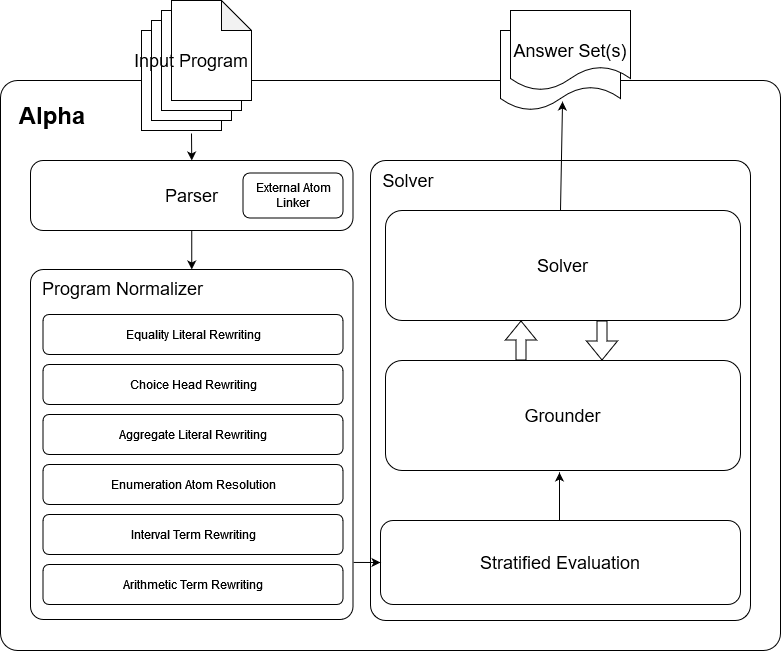
\includegraphics[width=\linewidth]{graphics/alpha-architecture.drawio.png}
    \caption{Alpha System Architecture}
    \label{fig:alpha-arch}
\end{figure}

\subsection{Parsing and Compilation}
\label{subsec:alpha-arch-compilation}

The core ground-and-solve component of Alpha supports only a subset of the input language described in Section~\ref{subsec:prelims-asp-syntax}. All language features supported by the parser, but not the solver itself, get compiled into equivalent constructs in the solver's internal representation. The following transformations are applied:
\begin{itemize}
    \item \emph{External Atom Linking}: Programs may only use external atoms whose implementations are known to the parser prior to parsing. Alpha provides a set of frequently used built-in external atoms out of the box, user-supplied code must be scanned through Alpha's API. Example~\ref{ex:user-supplied-externals} demonstrates the use of user-supplied atom definitions. All external atom implementations are linked during parsing, i.e. every external atom in the parsed program holds a reference to the implementing Java Method.
    \item \emph{Equality Literal Rewriting}: Literals like $A = B$ in rule bodies that establish an equality between variables are removed by replacing one variable with the other (e.g. $B$ with $A$ in the example). 
    \item \emph{Choice Head Rewriting}: Rules with a choice head get replaced by a set of rules and constriants that is semantically equivalent to the choice rule.
    \item \emph{Aggregate Literal Rewriting}: Aggregate literals like \texttt{N = \#count\{ X : interesting(X)\}} are replaced by a regular literal and a set of rules deriving instances of the replacement literal equivalent to the original aggregate literal. Subsection~\ref{subsubsec:alpha-arch-aggregate-rewriting} goes into more detail on the rewriting process.
    \item \emph{Enumeration Atom Resolution}: Alpha provides a feature where terms can be enumerated, i.e. the solver maps user-supplied terms to integers. This is used internally for Aggregate Literal Rewriting. Section~\ref{subsubsec:alpha-arch-enum-resolution} describes how the atoms in question are resolved.
    \item \emph{Interval Term Rewriting}: Interval terms, i.e. terms of form $A..B$ are transformed into regular variables that are bound through special internal literals which supply all values of the interval as ground instances of the variable.
    \item \emph{Arithmetic Term Rewriting}: In order to simplfy grounding later, terms constituting arithmetic expressions such as $p(f(X * 3, Y - 4))$ are rewritten such that no arithmetic expressions occur in nested terms, i.e. the atom from before would be rewritten to $p(f(R1, R2)), R1 = X * 3, R2 = Y - 4$.
\end{itemize}
The result of the above list of transformations is what is called a \emph{normalized} program in Alpha, which can directly be passed to the evaluation component and solved. Rewriting of Aggregate Literals and Resolution of Enumeration Atoms are of interest in the context of the Evolog reference implementation, and shall therefore be described in more detail.

\subsubsection{Enumeration Atoms}
\label{subsubsec:alpha-arch-enum-resolution}
Alpha permits use of an "enumeration" solver directive, which allows programs to associate terms with consecutive integer keys.
Listing~\ref{lst:enum-usage} demonstrates using an enumeration to assign integer ordinals to a set of colors. 
\begin{lstlisting}[style=asp-code, label={lst:enum-usage}, caption={Using the Enumeration Directive to enumerate color symbols.}]
#enumeration_predicate_is ordinal.

color(white). color(red). color(magenta).
color(yellow). color(green). color(cyan).
color(blue). color(black).
    
numbered_color(COL, NUM) :- 
    color(COL), ordinal(colors, COL, NUM).    
\end{lstlisting}    
The directive \texttt{\#enumeration\_predicate\_is} designates the predicate \texttt{ordinal/3} as an \emph{Enumeration Predicate}. All occurrences of the an enumeration predicate get replaced with a special internal predicate \texttt{\_Enumeration/3}. Listing~\ref{lst:enum-rewritten} shows the program from before after transformation.
\begin{lstlisting}[style=asp-code, label={lst:enum-rewritten}, caption={Transformed color numbering.}]
color(white). color(red). color(magenta).
color(yellow). color(green). color(cyan).
color(blue). color(black).

numbered_color(COL, NUM) :- 
    color(COL), _Enumeration(colors,COL,NUM).
\end{lstlisting} 
Alpha's grounding component calculates valid ground substitutions for enumeration atoms as follows: \\
Given an enumeration atom $a_e$ with terms $t_{enum}, t_{value}$ and $t_{ord}$ and a partial substitution $\sigma$, assigning ground values to $t_{enum}$ and $t_{value}$,
\begin{itemize}
    \item If the value $\sigma t_{enum}$ is encountered for the first time, initialize a new empty map (i.e. set of pairs with unique first elements), and associate it with  term $\sigma t_{enum}$.
    \item If the map for $\sigma t_{enum}$ does not contain a mapping for key $\sigma t_{value}$, extend $\sigma$ by the mapping $t_{ord} \mapsto o$, where $ = s + 1$ and $s$ denotes the current map size for $\sigma t_{enum}$. Add the mapping $(\sigma t_{ord}, o)$ to the map and return the extended version of $\sigma$.
    \item If a mapping for $\sigma t_{enum}$ and $\sigma t_{value}$ exists, read the associated ordinal $o$, add it to $\sigma$ and return the extended substitution.
\end{itemize}    
From a semantics point of view, enumeration literals can intuitively be seen as "lazily assigned fixed-interpretation literals"  (see Definition~\ref{def:prelims-asp-semantics-fixedinterpretation-literals}) in the way that every enumeration atom is true for exactly the ground substitution generated upon grounding it for the first time.

\subsubsection{Aggregate Atoms}
\label{subsubsec:alpha-arch-aggregate-rewriting}